\documentclass[aspectratio=169]{beamer}

\setbeamersize{text margin left=5mm, text margin right=5mm}

\defbeamertemplate{headline}{my header}{%
\vskip1pt%
\makebox[0pt][l]{\,\insertshortauthor}%
\hspace*{\fill}\insertshorttitle/\insertshortsubtitle\hspace*{\fill}%
\llap{\insertpagenumber/\insertpresentationendpage\,}
}
\setbeamertemplate{headline}[my header]

\let\olditem\item
\renewcommand{\item}{\setlength{\itemsep}{\fill}\olditem}

\usepackage{caption}
\usepackage{soul}
\usepackage{tkz-euclide}
\usetikzlibrary{calc}
\usepackage[]{algorithm2e}
\usepackage{changepage}
\usepackage{amssymb}
\usepackage{xcolor}
\usepackage{mathtools}
\usepackage{tcolorbox}
\usepackage{tikz}
\usepackage{tikz-3dplot}
\usetikzlibrary{arrows.meta, decorations.pathreplacing, positioning, shapes.geometric}

%% Fonts
\usefonttheme{professionalfonts}
\usefonttheme{serif}

\DeclareCaptionLabelFormat{blank}{}
\captionsetup[figure]{labelformat=blank}

%% Math definitions
\def\mf{\ensuremath\mathbf}
\def\mb{\ensuremath\mathbb}
\def\lp{\ensuremath\left(}
\def\rp{\ensuremath\right)}
\def\lv{\ensuremath\left\lvert}
\def\rv{\ensuremath\right\rvert}
\def\lV{\ensuremath\left\lVert}
\def\rV{\ensuremath\right\rVert}
\def\lc{\ensuremath\left\{}
\def\rc{\ensuremath\right\}}
\def\ls{\ensuremath\left[}
\def\rs{\ensuremath\right]}
\def\bmx{\ensuremath\begin{bmatrix*}[r]}
\def\emx{\ensuremath\end{bmatrix*}}
\def\bmxc{\ensuremath\begin{bmatrix*}[c]}
\def\t{\lp t\rp}
\def\k{\ls k\rs}

\newcommand{\demoex}[2]{\onslide<#1->\begin{color}{black!60} #2 \end{color}}
\newcommand{\demoexc}[3]{\onslide<#1->\begin{color}{#2} #3 \end{color}}
\newcommand{\anim}[3]{\onslide<#1->{\begin{color}{#2!60} #3 \end{color}}}
\newcommand{\ct}[1]{\lp #1\rp}
\newcommand{\dt}[1]{\ls #1\rs}
\newcommand{\cols}[2]{\begin{columns}[#1] #2 \end{columns}}
\newcommand{\col}[2]{\begin{column}{#1} #2 \end{column}}

%% Mycolors
\definecolor{myred}{RGB}{192,0,0}
\definecolor{mygray}{RGB}{100,100,100}

%% Custom beamer color
\setbeamercolor{title}{fg=myred}
\setbeamercolor{subtitle}{fg=myred}
\setbeamerfont{title}{series=\bfseries}
% \setbeamercolor{frametitle}{bg=myred, fg=white}
\setbeamercolor{frametitle}{bg=mygray!10!, fg=myred}
\setbeamerfont{frametitle}{series=\bfseries}
\setbeamercolor{item}{fg=mygray}
\setbeamercolor{title in head/foot}{fg=myred}

% Move header to footer
\setbeamertemplate{headline}{}
\setbeamertemplate{footline}{
  \begin{beamercolorbox}[wd=\paperwidth,ht=2.25ex,dp=1ex,center]{footline}
    \inserttitle\hfill\insertauthor\hfill\insertdate\hfill\insertframenumber{}
  \end{beamercolorbox}
}

\title{Applied Linear Algebra in Data Analysis}

% A subtitle is optional and this may be deleted
\subtitle{Matrices}

\author{Sivakumar Balasubramanian}
% - Give the names in the same order as the appear in the paper.
% - Use the \inst{?} command only if the authors have different
%   affiliation.

\institute[Christian Medical College] % (optional, but mostly needed)
{
  \inst{}%
  Department of Bioengineering\\
  Christian Medical College, Bagayam\\
  Vellore 632002
}
% - Use the \inst command only if there are several affiliations.
% - Keep it simple, no one is interested in your street address.

\date{}
% - Either use conference name or its abbreviation.
% - Not really informative to the audience, more for people (including
%   yourself) who are reading the slides online

\subject{Lecture notes on ALADA}
% This is only inserted into the PDF information catalog. Can be left
% out. 

% If you have a file called "university-logo-filename.xxx", where xxx
% is a graphic format that can be processed by latex or pdflatex,
% resp., then you can add a logo as follows:

% \pgfdeclareimage[height=0.5cm]{university-logo}{university-logo-filename}
% \logo{\pgfuseimage{university-logo}}

% Delete this, if you do not want the table of contents to pop up at
% the beginning of each subsection:
\AtBeginSubsection[]
{
  \begin{frame}<beamer>{Outline}
    \tableofcontents[currentsection,currentsubsection]
  \end{frame}
}

% Let's get started
\begin{document}

\begin{frame}
  \titlepage
\end{frame}

% \begin{frame}[t]{References}
% \begin{itemize}
% \item S Boyd, Applied Linear Algebra: Chapters 6, 7, 8, 10 and 11.
% \item G Strang, Linear Algebra: Chapters 1 and 2.
% \end{itemize}
% \end{frame}

\begin{frame}[t]{Matrices}
\begin{itemize}
\item \textbf{Matrices} are rectangular array of numbers. $\begin{bmatrix}
1.1 & -24 & \sqrt{2} \\
0 & 1.12 & -5.24 \\
\end{bmatrix}$
%\vspace{0.15cm}
\begin{center}
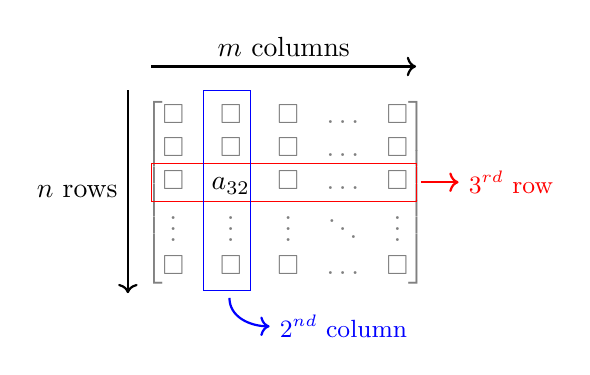
\begin{tikzpicture}[scale=0.6]
\draw[thick, ->] (0,0) -- (0, -4.3) node[midway,left] {$n$ rows};
\draw[thick, ->] (0.5,0.5) -- (6.1, 0.5) node[midway,above]{$m$ columns};
%\node[xshift=-0.6cm,yshift=-1.3cm] {Rows};
\node[gray,xshift=2.0cm,yshift=-1.3cm] {$\begin{bmatrix}
\Box & \Box & \Box & \ldots & \Box \\
\Box & \Box & \Box & \ldots & \Box \\
\Box & \textcolor{black}{a_{32}} & \Box & \ldots & \Box \\
\vdots & \vdots & \vdots & \ddots & \vdots \\
\Box & \Box & \Box & \ldots & \Box \\
\end{bmatrix}$};
\draw[draw=red] (0.5,-2.35) rectangle ++(5.6,0.8);
\draw[draw=blue] (1.6,-4.25) rectangle ++(1.0,4.25);
\draw [thick, blue, ->] (2.15,-4.4) to [out=-90,in=180] (3.0, -5.0) node[right] {\small{$2^{nd}$ column}};
\draw [thick, red, ->] (6.2,-1.95) to (7.,-1.95) node[right] {\small{$3^{rd}$ row}};
\end{tikzpicture}\hspace{0.5cm}
\end{center}
\item Consider a matrix $\mf{A}$ with $n$ rows and $m$ columns.$ \begin{cases} \text{\textbf{Tall/Skinny}} & n > m\\
\text{\textbf{Square}} & n = m\\
\text{\textbf{Wide/Fat}} & n < m\\
\end{cases}$
\end{itemize}
\end{frame}

\begin{frame}[t]{Matrices}
\begin{itemize}
    \item $n$-vectors can be interpreted as $n \times 1$ matrices. These are called \textit{column vectors}.
    \item A matrix with only one row is called a \textit{row vector}, which can be referred to as $n$-row-vector.  $\mf{x} = \begin{bmatrix}1.45 & -3.1 & 12.4\end{bmatrix}$
    \item\textbf{Block matrices} \& \textbf{Submatrices}: $\mf{A} = \begin{bmatrix}
    \mf{B} & \mf{C} \\
    \mf{D} & \mf{E}
    \end{bmatrix}$.  What are the dimensions of the different matrices?
\end{itemize}
\end{frame}


\begin{frame}[t]{Matrices}
\begin{itemize}
    \item Matrices are also compact way to give a set of indexed column $n$-vectors, 
    $\mf{x}_1, \mf{x}_2, \mf{x}_3 \ldots \mf{x}_m$. 
    $$\mf{X} = \begin{bmatrix}
    \mf{x}_1 & \mf{x}_2 & \mf{x}_3 & \ldots & \mf{x}_m
    \end{bmatrix}$$

    \item \textbf{Zero matrix}$ = \mf{0}_{n\times m} = \begin{bmatrix}
    0 & 0 & \ldots & 0\\
    0 & 0 & \ldots & 0\\
    \vdots & \vdots & \ddots & \vdots\\
    0 & 0 & \ldots & 0
    \end{bmatrix}$

    \item \textbf{Identity matrix} is a square $n \times n$ matrix with all zero elements, except the diagonals where all elements are 1.
    $$i_{mn} = \begin{cases}
    1 & m = n\\
    0 & m \neq n
    \end{cases} \,\,\,\,\,\,\,\, \mf{I}_3=\begin{bmatrix}
    1 & 0 & 0\\
    0 & 1 & 0\\
    0 & 0 & 1\\
    \end{bmatrix} = \begin{bmatrix}
    \mf{e}_1 & \mf{e}_2 & \mf{e}_3
    \end{bmatrix}$$
\end{itemize}
\end{frame}


\begin{frame}[t]{Matrices}
\begin{itemize}

\item \textbf{Diagonal matrices} is a square matrix with non-zero elements on its diagonal.
$$\begin{bmatrix}
0.4 & 0 & 0 & 0\\
0 & -11 & 0 & 0\\
0 & 0 & 21 & 0\\
0 & 0 & 0 & 9.3\\
\end{bmatrix} = \text{\textbf{diag}}\left(0.4, -11, 21, 9.3\right)$$
\item \textbf{Triangular matrices}: Are square matrices. \textit{Upper triangular} $a_{ij} = 0, \forall i > j$; \textit{Lower triangular} $a_{ij} = 0, \forall i < j$.
\end{itemize}
\end{frame}

\begin{frame}[t]{Matrix operations: Transpose}
\begin{itemize}
\item \textbf{Transpose} switches the rows and columns of a matrix. $\mf{A}$ is a $n\times m$ matrix, then its transpose is represented by $\mf{A}^{\top}$, which is a $m \times n$ matrix.
\[ \mf{A} = \begin{bmatrix}
a_{11} & a_{12} & a_{13}\\
a_{21} & a_{22} & a_{23}\\
\end{bmatrix} \implies \mf{A}^{\top} = \begin{bmatrix}
a_{11} & a_{21}\\
a_{12} & a_{22}\\
a_{13} & a_{23}\\
\end{bmatrix} \]
Transpose converts between column and row vectors.\\
What is the transpose of a block matrix? $\mf{A} = \begin{bmatrix}
\mf{B} & \mf{C}\\\mf{D} & \mf{E}
\end{bmatrix}$
\end{itemize}
\end{frame}

\begin{frame}[t]{Matrix operations: Matrix Addition}
\begin{itemize}
\item \textbf{Matrix addition} can only be carried out with matrices of same size. Like vectors we perform element wise addition.
\[ \begin{bmatrix}
a_{11} & a_{12}\\
a_{21} & a_{22}\\
\end{bmatrix} + \begin{bmatrix}
b_{11} & b_{12}\\
b_{21} & b_{22}\\
\end{bmatrix} = \begin{bmatrix}
a_{11} + b_{11} & a_{12} + b_{12}\\
a_{21} + b_{21} & a_{22} + b_{22}\\
\end{bmatrix}\]

\item \textbf{Properties of matrix addition}:
\begin{itemize}
\item \textit{Commutative}: $\mf{A} + \mf{B} = \mf{B} + \mf{A}$
\item \textit{Associative}: $\left(\mf{A} + \mf{B}\right) + \mf{C} = \mf{A} + \left(\mf{B} + \mf{C}\right)$
\item \textit{Addition with zero matrix}: $\mf{A} + \mf{0} = \mf{0} + \mf{A} = \mf{A}$
\item \textit{Transpose of sum}: $\left(\mf{A} + \mf{B}\right)^{\top} = \mf{A}^{\top} + \mf{B}^{\top}$
\end{itemize}
\end{itemize}
\end{frame}

\begin{frame}[t]{Matrix operations: Scalar multiplication}
\begin{itemize}
\item \textbf{Scalar multiplication} Each element of the matrix gets multiplied by the scalar.
\[ \alpha \begin{bmatrix}
a_{11} & a_{12}\\
a_{21} & a_{22}\\
\end{bmatrix} = \begin{bmatrix}
\alpha a_{11} & \alpha a_{12} \\
\alpha a_{21} & \alpha a_{22} \\
\end{bmatrix}\]
\item We will mostly only deal with matrices with real entries. Such matrices are elements of the set $\mathbb{R}^{n\times m}$.
\item Given the aforementioned matrix operations and their properties, is $\mathbb{R}^{n\times m}$ a vector space?
\end{itemize}
\end{frame}

\begin{frame}[t]{Matrix operations: Matrix multiplication}
\begin{itemize}
\item A useful multiplication operation can be defined for matrices.
\item It is possible to \textit{multiply} two matrices $\mf{A} \in \mathbb{R}^{n\times p}$ and $\mf{B} \in \mathbb{R}^{p\times m}$ through this \textit{matrix multiplication} procedure.
\item The product matrix $\mf{C} \coloneqq \mf{A}\mf{B} \in \mathbb{R}^{n \times m}$, if the number of columns of $\mf{A}$ is equal to the number of rows of $\mf{B}$.
\[ c_{ij} \coloneqq \sum_{k=1}^{p} a_{ik}b_{kj} \,\,\,\,\, \forall i \in \left\{1, \ldots n\right\}\,\,\, , j \in \left\{1 \ldots m\right\} \]
\end{itemize}
\end{frame}

\begin{frame}[t]{Matrix multiplication}
\begin{itemize}
\item \textit{Inner product} is a special case of matrix multiplication between a \textit{row vector} and a \textit{column vector}.
\[ \mf{x}^{\top}\mf{y} = \begin{bmatrix}
x_1 \\ x_2 \\ \vdots \\x_n
\end{bmatrix}^{\top}\begin{bmatrix}
y_1 \\ y_2 \\ \vdots \\y_n
\end{bmatrix} = \begin{bmatrix}
x_1 & x_2 & \ldots &x_n
\end{bmatrix}\begin{bmatrix}
y_1 \\ y_2 \\ \vdots \\y_n
\end{bmatrix} = \sum_{i=1}^nx_iy_i\]
\end{itemize}
\end{frame}

\begin{frame}[t]{Matrix multiplication: Post-multiplication by a column vector}
\begin{itemize}
\item Consider a matrix $\mf{A} \in \mathbb{R}^{n \times m}$ and a $m$-vector $\mf{x} \in \mathbb{R}^m$. We can multiply $\mf{A}$ and $\mf{x}$ to obtain $\mf{y} = \mf{A}\mf{x} \in \mathbb{R}^n$.
\[ \mf{y} = \begin{bmatrix}
a_{11} & a_{12} & \ldots & a_{1m} \\
a_{21} & a_{22} & \ldots & a_{2m} \\
\vdots & \vdots & \ddots & \vdots \\
a_{n1} & a_{n2} & \ldots & a_{nm} \\
\end{bmatrix}\begin{bmatrix}
x_1\\ x_2 \\ \vdots \\ x_{m}
\end{bmatrix} = \begin{bmatrix}
\sum_{i=1}^ma_{1i}x_i\\ \sum_{i=1}^ma_{2i}x_i \\ \vdots \\ \sum_{i=1}^ma_{ni}x_i
\end{bmatrix} = \sum_{i=1}^mx_i\begin{bmatrix}
a_{1i} \\ a_{2i} \\ \vdots \\ a_{ni}
\end{bmatrix} = \sum_{i=1}^mx_i \mathbf{a}_{i} \]
\item Post-multiplying a matrix $\mf{A}$ by a column vector $\mf{x}$ results in a linear combination of the columns of matrix $\mf{A}$.

\item $\mathbf{x}$ provides the column mixture.
\end{itemize}
\end{frame}

\begin{frame}[t]{Matrix multiplication: Pre-multiplication by a row vector}
\begin{itemize}
\item Let $\mf{x}^{\top} \in \mathbb{R}^{n}$ and $\mf{A} \in \mathbb{R}^{n \times m}$, then $\mf{y} = \mf{x}^{\top}\mf{A}$.
\[ \mf{y} = \begin{bmatrix}
x_1 & \ldots & x_n
\end{bmatrix} \begin{bmatrix}
a_{11} & \ldots & a_{1m} \\
\vdots & \ddots & \vdots \\
a_{n1} & \ldots & a_{nm} \\
\end{bmatrix} = \begin{bmatrix} \sum_{i=1}^{n} x_i a_{i1} & \ldots & \sum_{i=1}^{n} x_i a_{im}
\end{bmatrix} = \sum_{i=1}^n x_i \tilde{\mf{a}}_i^\top \]
where, $\tilde{\mf{a}}_i^\top = \begin{bmatrix}
a_{i1} & \ldots & a_{im}\end{bmatrix}$
\item Pre-multiplying a matrix $\mf{A}$ by a row vector $\mf{x}$ results in a linear combination of the rows of $\mf{A}$.

\item $\mf{x}^\top$ provides the row mixture.
\end{itemize}
\end{frame}

\begin{frame}[t]{Matrix multiplication}
\begin{itemize}
\item Multiplying two matrices $\mf{A} \in \mathbb{R}^{n \times p}$ and $\mf{B} \in \mathbb{R}^{p \times m}$ produces $\mf{C} \in \mathbb{R}^{n \times m}$,
\[ \mf{C} = \mf{A}\mf{B} = \begin{bmatrix}
a_{11} & a_{12} & \ldots & a_{1p} \\
a_{21} & a_{22} & \ldots & a_{2p} \\
\vdots & \vdots & \ddots & \vdots \\
a_{n1} & a_{n2} & \ldots & a_{np} \\
\end{bmatrix} \begin{bmatrix}
b_{11} & b_{12} & \ldots & b_{1m} \\
b_{21} & b_{22} & \ldots & b_{2m} \\
\vdots & \vdots & \ddots & \vdots \\
b_{p1} & b_{p2} & \ldots & b_{pm} \\
\end{bmatrix} = \begin{bmatrix}
c_{11} & c_{12} & \ldots & c_{1m} \\
c_{21} & c_{22} & \ldots & c_{2m} \\
\vdots & \vdots & \ddots & \vdots \\
c_{p1} & c_{n2} & \ldots & c_{nm} \\
\end{bmatrix}\]

\item \textbf{Four interpretations of matrix multiplication.}
\begin{enumerate}
  \item Inner-Product interpretation
  \item Column interpretation
  \item Row interpretation
  \item Outer product interpretation.
\end{enumerate} 
\end{itemize}
\end{frame}

\begin{frame}[t]{Matrix multiplication: Inner-product Interpreation}
\[ \mf{C} = \mf{A}\mf{B}, \,\,\, \mf{A} \in \mathbb{R}^{n \times p}, \, \mf{B} \in \mathbb{R}^{p \times m}, \, \mf{C} \in \mathbb{R}^{n \times m} \]
\begin{itemize}
\item $ij^{th}$ element of $\mf{C}$ is the inner product of the $i^{th}$ row of $\mf{A}$ and the $j^{th}$ column of $\mf{B}$.
 \[ c_{ij} = \sum_{k=1}^{p} a_{ik} b_{kj} = \tilde{\mf{a}}_i^{\top}\mf{b}_j \]
 where, $i \in \left\{1 \ldots n\right\}, j \in \left\{1 \ldots m\right\}$
\end{itemize}
\end{frame}


\begin{frame}[t]{Matrix multiplication: Column interpretation}
\[ \mf{C} = \mf{A}\mf{B}, \,\,\, \mf{A} \in \mathbb{R}^{n \times p}, \, \mf{B} \in \mathbb{R}^{p \times m}, \, \mf{C} \in \mathbb{R}^{n \times m} \]
\begin{itemize}
\item Columns of $\mf{C}$ are the linear combinations of the columns of $\mf{A}$.
\[ \mf{C} = \mf{A} \begin{bmatrix}
\mf{b}_{1} & \mf{b}_{2} & \ldots & \mf{b}_{m}
\end{bmatrix} = \begin{bmatrix}
\mf{A}\mf{b}_{1} & \mf{A}\mf{b}_{2} & \ldots & \mf{A}\mf{b}_{m}
\end{bmatrix} \]

\item $j^{th}$ column of $\mf{C}$ is the linear combination of the columns of $\mf{A}$
\[ \mf{c}_j = \sum_{k=1}^{p} b_{kj} \mf{a}_k \]
\end{itemize}
\end{frame}


\begin{frame}[t]{Matrix multiplication: Row interpretation}
\[ \mf{C} = \mf{A}\mf{B}, \,\,\, \mf{A} \in \mathbb{R}^{n \times p}, \, \mf{B} \in \mathbb{R}^{p \times m}, \, \mf{C} \in \mathbb{R}^{n \times m} \]
\begin{itemize}
\item Rows of $\mf{C}$ are the linear combinations of the rows of $\mf{B}$.
\[ \mf{C} = \begin{bmatrix}
\tilde{\mf{a}}_{1}^\top \\ \tilde{\mf{a}}_{2}^\top \\ \ldots \\ \tilde{\mf{a}}_{n}^\top
\end{bmatrix} \mf{B}  = \begin{bmatrix}
\tilde{\mf{a}}_{1}^\top \mf{B} \\ \tilde{\mf{a}}_{2}^\top \mf{B} \\ \ldots \\ \tilde{\mf{a}}_{n}^\top \mf{B}
\end{bmatrix} \]

\item $i^{th}$ row of $\mf{C}$ is the linear combination of the rows of $\mf{B}$
\[ \tilde{\mf{c}}_i^\top = \sum_{k=1}^{p} a_{ik} \tilde{\mf{b}}_{k}^\top  \]
\end{itemize}
\end{frame}


\begin{frame}[t]{Matrix multiplication: Outer product interpretation}
\begin{itemize}
    \item \textbf{Outer product}: Product between a colum vector and a row vector. Let $\mf{x} \in \mathbb{R}^n$ and $\mf{y} \in \mathbb{R}^m$. The \textit{outer product} is defined as,
    \[ \mf{x}\mf{y}^{\top} = \begin{bmatrix}
    x_1\\ x_2\\ \vdots \\x_n
    \end{bmatrix} \begin{bmatrix}
    y_1 &  y_2 & \ldots & y_m
    \end{bmatrix} = \begin{bmatrix}
    x_1y_1 &  x_1y_2 & \ldots & x_1y_m \\
    x_2y_1 &  x_2y_2 & \ldots & x_2y_m \\
    \vdots &  \vdots & \ddots & \vdots \\
    x_ny_1 &  x_ny_2 & \ldots & x_ny_m \\
    \end{bmatrix} \in \mb{R}^{n \times m} \]
\end{itemize}
\end{frame}


\begin{frame}[t]{Matrix multiplication: Outer product interpretation}
\[ \mf{C} = \mf{A}\mf{B}, \,\,\, \mf{A} \in \mathbb{R}^{n \times p}, \, \mf{B} \in \mathbb{R}^{p \times m}, \, \mf{C} \in \mathbb{R}^{n \times m} \]
\begin{itemize}
    \item $\mf{C}$ can be written as the sum of $p$ outer products of columns of $\mf{A}$ and rows of $\mf{B}$.
    \[ \mf{C} = \mf{A}\mf{B} = \begin{bmatrix}
    \mf{a}_1 & \mf{a}_2 & \mf{a}_3 & \ldots & \mf{a}_p
    \end{bmatrix} \begin{bmatrix}
    \tilde{\mf{b}}_1^{\top} \\
    \tilde{\mf{b}}_2^{\top} \\
    \tilde{\mf{b}}_3^{\top} \\
    \vdots \\
    \tilde{\mf{b}}_p^{\top}
    \end{bmatrix} = \sum_{i=1}^{p}\mf{a}_i\tilde{\mf{b}}_i^{\top} \]
\end{itemize}
\end{frame}


\begin{frame}[t]{Properties of matrix multiplication}
\begin{itemize}
\item \textbf{Not commutative}: $\mf{A}\mf{B} \neq \mf{B}\mf{A}$\\
The product of two matrices might not alwasys be defined. When it is defined, $\mf{A}\mf{B}$ and $\mf{B}\mf{A}$ need not match.
\item \textbf{Distributive}:  $\mf{A}\left(\mf{B} + \mf{C}\right) = \mf{A}\mf{B} + \mf{B}\mf{C}$ and $\left(\mf{A} + \mf{B}\right)\mf{C} = \mf{A}\mf{C} + \mf{B}\mf{C}$ 
\item \textbf{Associative}: $\mf{A}\left(\mf{B}\mf{C}\right) = \left(\mf{A}\mf{B}\right)\mf{C} $
\item \textbf{Transpose}: $\left(\mf{A}\mf{B}\right)^{\top} = \mf{B}^{\top}\mf{A}^{\top}$
\item \textbf{Scalar product}: $\alpha\left(\mf{A}\mf{B}\right) = \left(\alpha \mf{A}\right)\mf{B} = \mf{A}\left(\alpha \mf{B}\right)$
\end{itemize}
\end{frame}


\begin{frame}[t]{Linear transformations}
  \begin{itemize}
      \item Linear functions $f: \mathbb{R}^m \mapsto \mathbb{R}$, 
      $$y = f\left(\mf{x}\right) = \mf{w}^{\top}\mf{x}; \,\,\, \mf{w}, \mf{x} \in \mathbb{R}^m, \,\, y \in \mathbb{R}$$
  
      \item Generalization of the linear function is when its range $\mathbb{R}^n$:
      $$\mf{y} = f\left(\mf{x}\right); \,\,\, \mf{x} \in \mathbb{R}^m, \,\, \mf{y} \in \mathbb{R}^n$$
  
      \item These can be represented as, $\mf{y} = \mf{Ax}, \,\,\, \mf{A} \in \mathbb{R}^{n \times m}$.\\
  
      \item Matrices can be thought of as representing a particular linear transformation.
  \end{itemize}
\end{frame}


\begin{frame}[t]{Why does matrix multiplication have this strange definition?}
  Consider the following two functions,
  \begin{small}
  \[ \mf{y} = f\lp\mf{x}\rp = \mf{A}\mf{x} \longrightarrow \begin{bmatrix}y_1 \\ y_2\end{bmatrix} = f\left(\begin{bmatrix}x_1 \\ x_2\end{bmatrix}\right) = \begin{bmatrix}ax_1 + bx_2 \\ cx_1 + dx_2\end{bmatrix} = \begin{bmatrix}a & b \\ c & d\end{bmatrix}\begin{bmatrix}x_1 \\ x_2\end{bmatrix}\]
  \[ \mf{v} = g\lp\mf{u}\rp = \mf{B}\mf{u} \longrightarrow \begin{bmatrix}v_1 \\ v_2\end{bmatrix} = g\left(\begin{bmatrix}u_1 \\ u_2\end{bmatrix}\right) = \begin{bmatrix}\alpha u_1 + \beta u_2 \\ \gamma u_1 + \delta u_2\end{bmatrix} = \begin{bmatrix}\alpha & \beta \\ \gamma & \delta\end{bmatrix}\begin{bmatrix}u_1 \\ u_2\end{bmatrix}\]
  \[ \begin{split}
  \mf{z} = h\left(\mf{u}\right) &= f\left(g\left(\mf{u}\right)\right) = f\left(\begin{bmatrix}\alpha u_1 + \beta u_2 \\ \gamma u_1 + \delta u_2\end{bmatrix}\right) = \begin{bmatrix}a\alpha u_1 + a\beta u_2 + b\gamma u_1 + b\delta u_2 \\ c\alpha u_1 + c\beta u_2 + d\gamma u_1 + d\delta u_2 \end{bmatrix}\\
  &= \begin{bmatrix}\left(a\alpha + b\gamma\right) u_1 + \left(a\beta + b\delta\right)u_2 \\ \left(c\alpha + d\gamma\right)u_1  + \left(c\beta + d\delta\right)u_2 \end{bmatrix} = \begin{bmatrix}a\alpha + b\gamma & a\beta + b\delta \\ c\alpha + d\gamma & c\beta + d\delta \end{bmatrix} \begin{bmatrix}u_1 \\ u_2 \end{bmatrix}
  \end{split}
  \]
  \[\mf{z} = \mf{A}\lp\mf{B}\mf{u}\rp = \lp\mf{A}\mf{B}\rp\mf{u} \implies \mf{A}\mf{B} = \begin{bmatrix}a & b \\ c & d\end{bmatrix}\begin{bmatrix}\alpha & \beta \\ \gamma & \delta\end{bmatrix} = \begin{bmatrix}a\alpha + b\gamma & a\beta + b\delta \\ c\alpha + d\gamma & c\beta + d\delta \end{bmatrix}
  \]
  \end{small}
  Matrix multiplication represents the composition of linear transformations.
\end{frame}


\begin{frame}[t]{Rank of a matrix $\mf{A}$}
  \begin{itemize}
  \item \textbf{Rank of a matrix $\mf{A}$}: dimension of the subspace spanned by the columns of $\mf{A}$ or the rows of $\mf{A} \in \mb{R}^{n \times m}$. 
  \[ \begin{split} 
  rank\lp \mf{A} \rp &= \mathrm{dim} \, span\lp \lc \mf{a}_1, \mf{a}_2, \ldots \mf{a}_m \rc \rp \rightarrow \text{Column rank}\\ 
  &= \mathrm{dim} \, span\lp \lc \tilde{\mf{a}}_1^\top, \tilde{\mf{a}}_2^\top, \ldots \tilde{\mf{a}}_n^\top \rc \rp \rightarrow \text{Row rank}
  \end{split}
  \]
  
  \item Column Rank is always equal to the row rank.
  
  \item Rank tells us the number of independent columns/rows in the matrix.
  
  \item \textbf{Full rank matrix } $\mf{A}$: $rank\lp \mf{A} \rp  = \min\lp n, m\rp$\\
        \textbf{Rank deficient matrix } $\mf{A}$: $rank\lp \mf{A} \rp  < \min\lp n, m\rp$
  \end{itemize}
  \end{frame}
    
\begin{frame}[t]{Matrix Inverse}
  \begin{small}
  \begin{itemize}
      \item Consider the square matrix $\mf{A} \in \mathbb{R}^{n \times n}$. $\mf{B} \in \mathbb{R}^{n \times n}$ is the inverse of $\mf{A}$, if $\mf{AB} = \mf{BA} = \mf{I}_n$, and $\mf{B}$ is represented as $\mf{A}^{-1}$.
      \item Not all matrices have inverses. A matrix with an inverse is called \textbf{non-singular}, otherwise it is called \textbf{singular}.
      \item For a non-singular matrix $\mf{A}$, $\mf{A}^{-1}$ is unique. $\mf{A}^{-1}$ is both the left and right inverse.
      \item A matrix $\mf{A}$ has an inverse, if and only if $\mf{A}$ is full rank, i.e. $rank\left(\mf{A}\right) = n$
      \item $\mf{Ax} = \mf{b}$ can be solved as follows, $\mf{x} = \mf{A}^{-1}\mf{b}$. \textit{It is never solved like this in practice.}
      \item Inverse of product of matrices, $\left(\mf{AB}\right)^{-1} = \mf{B}^{-1}\mf{A}^{-1}$.
      \item $\left(\mf{A}^{-1}\right)^{-1} = \mf{A}$ and $\left(\mf{A}^{-1}\right)^{\top} = \left(\mathbf{A}^{\top}\right)^{-1}$
\end{itemize}
\end{small}
\end{frame}


\begin{frame}[t]{Complex Vectors and Matrices}
  \begin{itemize}
      \item Similar to $\mb{R}^n$, we can have $\mb{C}^n$. $\mf{x} = \begin{bmatrix*}x_{1}\\x_{2}\\\vdots\\x_{n}\end{bmatrix*} = \begin{bmatrix*}x_{r1} + jx_{i1}\\x_{r2} + jx_{i2}\\\vdots\\x_{rn} + jx_{in}\end{bmatrix*}$
      
      \item Vector addition and scalar mulitplication are the same. The scalar is a complex number.
      
      \item Additive identity, and scalar multiplication identity are the same. So is the \textbf{standard basis} $\left\{\mf{e}_i\right\}_{i=1}^{n}$
      
      \item \textbf{Linear independence}: The set $\left\{\mf{v}_i\right\}_{i=1}^n$ with $\mf{v}_i \in \mb{C}^n$ is linearly independent, if  $\sum_{i=1}^nc_i\mf{v}_i = 0, \implies c_i = 0, \,\, \forall 1 \leq i \leq n, \,\,\, c_i \in \mb{C}$
      
      \item \textbf{Inner product}: $\mf{x}^{*}\mf{y} = \begin{bmatrix*}\overline{x}_1&\overline{x}_2&\ldots&\overline{x}_n\end{bmatrix*}\begin{bmatrix*}y_1\\y_2\\\vdots\\y_n\end{bmatrix*} = \sum_{i=1}^n\overline{x}_iy_i$
  
  \end{itemize}
  \end{frame}
  
  
  \begin{frame}[t]{Complex Vectors and Matrices}
  \begin{itemize}
      \item \textbf{Length}: $\Vert \mf{x} \Vert_2^2 = \mf{x}^{*}\mf{x} = \sum_{i=1}^n\overline{x}_ix_i = \sum_{i=1}^n\left\lvert x_i\right\rvert^2$
  
      \item \textbf{Orthogonality}: $\mf{x}^{*}\mf{y} = 0$
  
      \item Complex matrices have complex entries. $\mf{A} \in \mb{C}^{m \times n}$ such that $a_{ij} \in \mb{C}, \,\, \forall 1 \leq i \leq m, \,\, 1 \leq j \leq n$
  
      \item The transpose operation is generalized to conjugate transpose known as the \textit{Hermitian}. $\mf{A}^{*} = \overline{\mf{A}}^\top$.
      
      \item The idea of symmetric matrices $\mb{R}^{n \times n}$ are now generalized to $\mb{C}^{n \times n}$  as $\mf{A} = \mf{A}^{*}$. Such matrices are called \textbf{Hermitian} matrices.
  
      \item Orthogonal matrices in the complex case are called \textbf{Unitary} matrices, $\mf{U}^{*}\mf{U} = \mf{I} \implies \mf{U}^{-1} = \mf{U}^{*}$.
  \end{itemize}
  \end{frame}


\end{document}